\documentclass{article}
\usepackage{amsmath}
\usepackage{tikz}
\begin{document}

\subsection*{Gestion De Proyectos}
\textit{18. En el problema de gestión de proyectos tenemos un proyecto que se divide en $n$ etapas $v_1, \ldots, v_n$. Cada etapa $v_i$ consume un tiempo $t_i \geq 0$. Para poder empezar una etapa $v_i$, se requiere que primero se hayan terminado un conjunto $N(v_i)$ de etapas $v_j$ tales que $j < i$. Por simplicidad, la etapa $v_1$ se usa como indicador de inicio del proyecto y, por lo tanto, consume un tiempo $t_1 = 0$ y es requerida por todas las otras etapas. Análogamente, la etapa $v_n$ indica el final del proyecto, por lo que consume tiempo $t_n = 0$ y requiere la finalización del resto de las etapas. Una etapa es crítica cuando cualquier retraso en la misma provoca un retraso en la finalización del proyecto. Modelar el problema de encontrar todas las etapas críticas de un proyecto como un problema de camino mínimo e indicar qué algoritmo usaría para resolverlo. El mejor algoritmo que conocemos toma tiempo lineal en la cantidad de datos necesarios para describir un proyecto.} \\

Vamos a construir un digrafo, en el cual nuestros vértices son nuestras $v_i$ etapas. Las aristas están dadas por los requisitos de cada etapa, es decir, si la etapa $v_3$ requiere de $v_2$ y $v_0$, entonces existen las aristas $v_2 \to v_3$ y $v_0 \to v_3$. Los costos en cada arista están dados por el costo del nodo de llegada; en la arista $(v_2, v_3)$ el costo es $t_3$.


\begin{figure}[h]


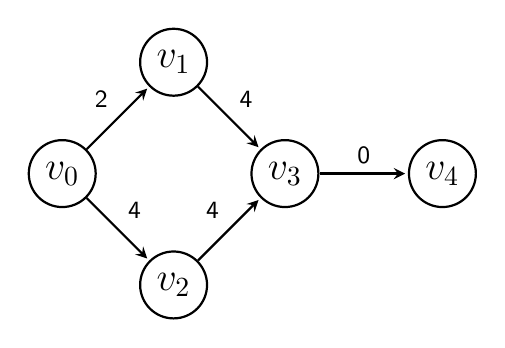
\begin{tikzpicture}[->,>=stealth,shorten >=1pt,auto,node distance=2cm,
                    thick,main node/.style={circle,draw,font=\sffamily\Large\bfseries}]

  \node[main node] (v0) {$v_0$};
  \node[main node] (v1) [above right of=v0] {$v_1$};
  \node[main node] (v2) [below right of=v0] {$v_2$};
  \node[main node] (v3) [below right of=v1] {$v_3$};
  \node[main node] (v4) [right of=v3] {$v_4$};

  \path[every node/.style={font=\sffamily\small}]
    (v0) edge node {2} (v1)
         edge node {4} (v2)
    (v1) edge node {4} (v3)
    (v2) edge node {4} (v3)
    (v3) edge node {0} (v4);
\end{tikzpicture}
\caption{Grafo de proyecto, con v3 dependiendo de v2 y v1. Se observa que  v2 es una tarea critica}
\end{figure}



Sobre este grafo, nuestras tareas críticas son aquellas que pertenecen a caminos máximos desde la tarea inicial (nuestra raíz) hasta la tarea final. Necesitamos identificarlos. Para eso usaremos una función similar a la del ejercicio 16, pero en lugar de minimizar, buscamos maximizar. Formalmente, los caminos máximos hasta $v_0$ están dados por:
\[
d(w) = \begin{cases} 
0 & \text{si } w = v_0 \\
\max_{z \in N^-(w)} (c(z,w) + d(z)) & \text{para } w \neq v_0
\end{cases}
\]

Luego, para reconstruir cuáles pertenecen al camino máximo, usamos un criterio similar al de $s$-$t$ eficiente, pero esta vez en caminos máximos. Es decir, necesitamos usar esta función, con caso base $0$ si $w = v_n$, sobre el DAG transpuesto, para obtener la distancia máxima de todos a $w$.

Con estos dos vectores de distancias precalculados, podemos recorrer todas las aristas en $O(m)$ y verificar si pertenecen o no al camino máximo, obteniendo así las tareas críticas.

Complejidad: $2 \cdot O(n+m) + O(m) = O(n + m)$.

\end{document}
